\chapter*{Preface}

Medicine has always been a scientific area where the crossing of different fields of research accounted for breakthroughs leading to a better understanding and, consequently, improved therapeutic methods.
The success of modern approaches and the development future techniques owes to the increased interdisciplinary research and work done by both medical personnel such as doctors and nurses, but also scientists like biologists, chemists, physicists and engineers.
As the knowledge about our own human body grows, the problems that we face are becoming more and more complex and need the interdisciplinary expertise.
Even though some therapeutic questions appear easy to answer, because they are easily understood on a general level, the actual treatment of a real patient is something entirely different.
Coming up with a treatment plan becomes exceedingly complex as we try to improve its precision and go towards targeted therapies which are tailor fit to the needs of an individual patient.
Improving their quality of life and chance of survival has always come with increased costs and effort as trade-off.
To make the best treatments available for everyone and, in the long run, also reduce the cost of used resources:
This work shall be a small contribution to this development.

\chapter{Introduction}
\label{chap:intro}
% o General: Start with very general description and focus step by step on your topic
% o keep in mind, that the introduction usually contains the most references
% o Introduction to main topic (e.g. Radiotherapy, MRI, ...) including historical review (1-2pages), Purpose of Radiotherapy ; Regardless of your actual topic, put it in context to conventional photon radiotherapy
% o Basic principles of Physics related to your topic
% o (e.g. Photo effect, Compton effect, Bethe-Bloch equation, ...)
% o Technological Background related to your topic
% o Give a general descriptions about the devices used in your thesis
% o (e.g. Linac, Afterloader, Synchrotron, Detectors...)
% o Overview of literature connected to your topic
% o Purpose of the thesis
% o based on the literature research, describe which information is missing, describe briefly what your thesis is about and what is the novelty of your work



\section{Photon - matter interactions}
\label{sec:photon}

As light (visible and invisible wavelengths) passes through matter, its intensity decreases.
This phenomenon is due to photons interacting with electrons, nuclei and their electric fields.
All processes either change the direction they travel in, alter their energy, or result in the disappearance of single photons.
The probability of these interactions differ for each material (dependent on its density; proton number $Z$) and photon energy ($h\nu$). \\

If a photon's energy exceeds the binding energy of an orbital electron, the photoelectric interaction can occur.
Also known as 'photo effect', it describes a photon being completely absorbed by a tightly bound orbital electron which then is ejected from its atom.
The now free electron is called 'photo-electron'. Its kinetic energy is the difference of the photon's energy and the electron's binding energy:
\begin{align}
E_{kin} &= h\nu - E_{binding}
\end{align} \\

Instead of being absorbed, photons might also just 'bounce off' electrons or entire atoms, transferring momentum and, in some cases, part of their energy to the particle they collide with.
Rayleigh (coherent) scattering happens when a photon interacts with a tightly bound orbital electron (transferring momentum to the entire atom).
This event can be seen as elastic, because only a negligible part of the photon's energy is transferred.

The Compton effect (incoherent scattering) involves a essentially free electron, such as an orbital electron with a relatively small binding energy compared to the photon's energy.
Due to the weak binding, momentum is transferred only to the electron.
This 'recoil electron' (or 'Compton electron') leaves its atom with a significant kinetic energy, which originated from the scattered photon.
Since the photon loses part of its energy, the event is considered inelastic. \\

When a photon with an energy above $1.022 \, MeV$ passes through the electric field of a nucleus, it might disappear to create an electron-positron pair.
This effect is called pair production.
The threshold of $1.022 \, MeV$ equals exactly the rest mass $E_m = 2m_ec^2$ for the two equally heavy particles (electron and positron).
The new particles travel in opposite directions with the same kinetic energy:
\begin{align}
 E_{kin} = \frac{h\nu - 1.022 \, MeV}{2}
\end{align} \\

A photon with energy of the order of $2 \, MeV$ or higher can also interact directly with the nucleus.
Such a Photonuclear reaction is similar to the photo effect, in the sense that the photon is completely absorbed.
Its energy is transferred to the nucleus resulting in the emission of either a proton or neutron.

\subsubsection{Attenuation}
The aforementioned interactions result in a gradual decrease of radiation intensity as it travels through matter.
The combined effect is described by Beer's law:
\begin{align}
I(x) = I_0 e^{-\mu(h\nu,Z)x}
\end{align}

where $x$ is the thickness of a homogeneous material and $\mu$ its linear attenuation coefficient.
The different probabilities for the interactions to occur is implicitly considered by the attenuation coefficient $\mu(h\nu,Z)$ (see Figure \ref{fig:attenuation_iron}).

For a photon being transmitted through matter with varying properties, the attenuation coefficient changes, too.
After travelling a distance $d$, the intensity can be expressed as:
\begin{align}
\label{eq:mu_int}
%I(x) = I_0 e^{- \int_{0}^{d} \mu(x)dx}
\end{align}

Where $\mu(x)$ describes the attenuation at every distance $x$.
(For whole chapter \ref{sec:photon}: \cite{Podgorsak, Maidment2014})

\begin{figure}[h!]
	\centering
	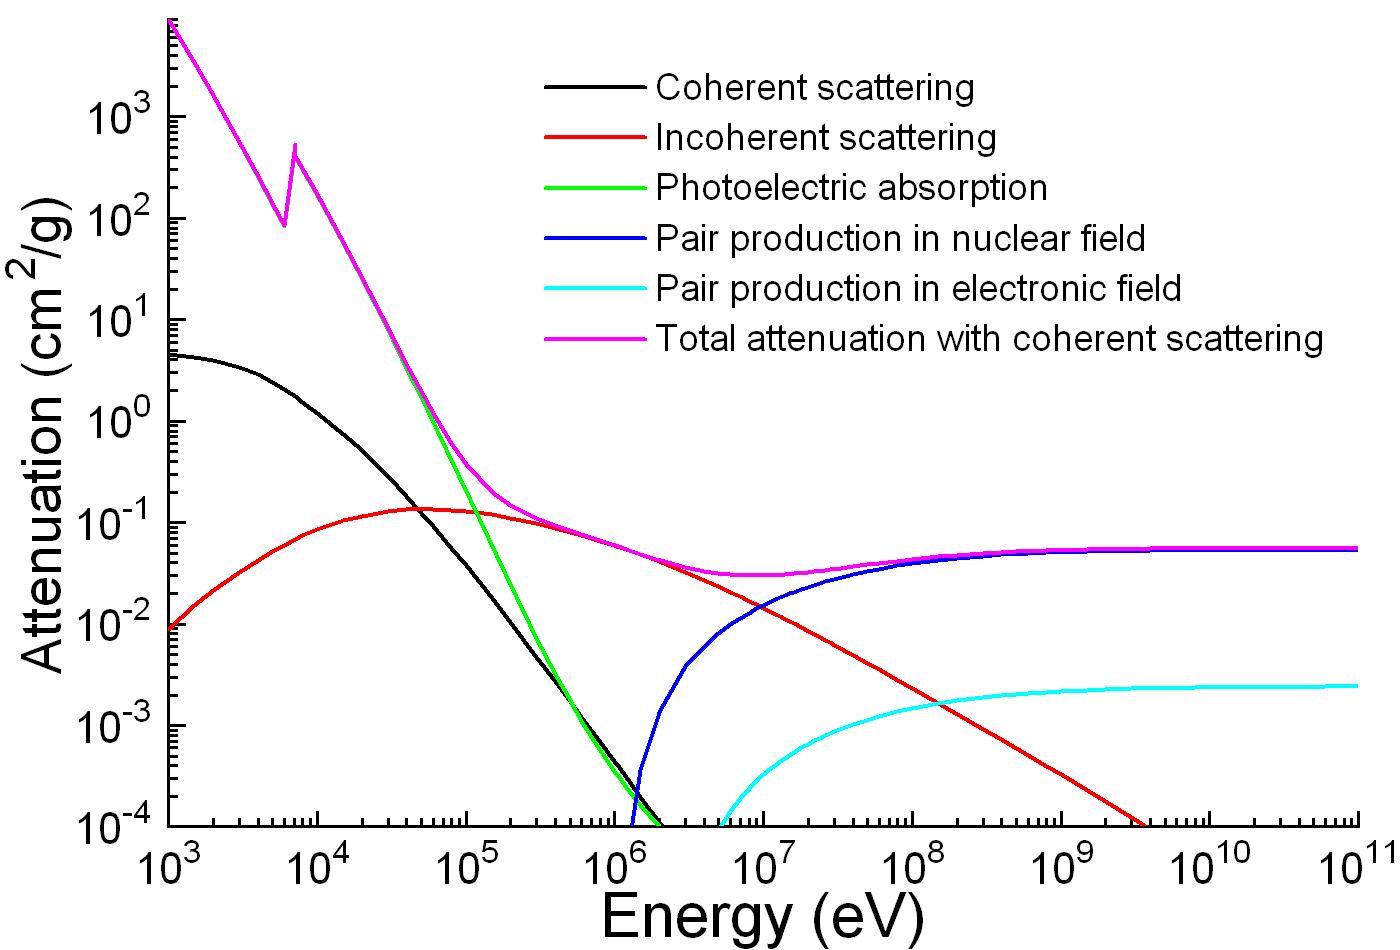
\includegraphics[width=0.7\linewidth]{../fig/intro/Ironattenuation}
	\caption{Photon attenuation for iron; \cite{Materialscientist}}
% source: by 'Materialscientist', via Wikimedia Common %(\url{https://commons.wikimedia.org/wiki/File:Ironattenuation.PNG?uselang=en})\\ GFDL %(\url{http://www.gnu.org/copyleft/fdl.html})\\ CC BY-SA 3.0 (\url{http://creativecommons.org/licenses/by-sa/3.0})
	\label{fig:attenuation_iron}
\end{figure}

\section{Basics of Radiobiology}
\label{sec:cell}
\subsection{The human cell}
All higher organisms consist of cells working together to form what is called tissue.
A collection of tissues which perform one or more functions is considered an organ. \\

Even though different types of cells exhibit distinctive traits which set them apart, all of them originated from the same totipotent zygote containing a original set of DNA.
A zygote is a stem cell, it has the ability to replicate indefinitely, passing its DNA on to the resulting daughter cells.
At the same time, it can change into any type of body cell. This feature is why it is called 'totipotent'.
As soon as the zygote has divided into a sufficient number of identical cells, all of them differentiate into the various human tissues.
In favour of becoming more specialised, cells lose their totipotency.
During the early stages of an embryo they are still capable of developing into a number of different cell types, but already restricted to their own tissue type; either nerve, skin, or blood \& muscle tissue.
As those cells further specialise, they limit their potential even more.
In a fully grown human body there are still stem cells present, such as bone marrow stem cells.
Other than the zygote, bone marrow can only give rise to blood cells, but not to e.g. nerve or skin cells.
A blood cell itself cannot replicate, it is considered a 'mature cell'.

The whole process follows guidelines dictated by the DNA.
Every cell inherited its own personal copy of the original set.
Inevitably, mistakes happen during its replication resulting in changes to the DNA called 'mutation'.
Most of these alterations are repaired or do not lead to changes in the cells behaviour.

The time needed for a reparation process to be completed is not the same as the period between cell reproduction. Changes to the DNA (e.g. mutations) occurring less frequently than one reparation cycle are less probable to result in permanent alterations, than those taking place more frequently. This is the reason why cells in tissues and organs that divide more frequently (i.e. gonads) are more prone to cancer development than those reproducing more slowly (i.e. bones).

As the human body ages, the repair mechanism loses some of its efficiency and mutations accumulate.
At one point, a cell may be reprogrammed to act in a unpredictable way, giving up its duties and duplicating without restraint, possibly forming tumours.
Also, external factors are known to influence cell behaviour and induce such 'malign' cells (carcinogenesis).
Cancer cells usually replicate more frequent than healthy cells, eventually leading to characteristic symptoms.

Different approaches have been developed to treat cancer, not all of which are suited to tackle every type of tumour.
If the tumour's location is unknown or metastases have formed already in many places, chemotherapy might be considered.
An easily accessible tumour could be removed in a surgery.
Non invasive therapies also include radiotherapy, destroying cancer cells using radiation. (see chapter \ref{sec:irradiate}.)

Generally, early treatments have high chances of success, but tumours are often not noticed until they reached a certain stage. 
Reliable ways of diagnosing tumours are made possible by imaging techniques visualising the interior of the human body. \cite{Baumann2017, Basic Clinical Radiobiology (4th edition)}

\subsection{Effects of radiation}
\label{sec:irradiate}

Cell damage could either be caused by radiation interacting directly with the critical target in a cell or with other molecules and atoms within the cell.
For X-rays, two thirds of the biological damage is attributed to indirect action.
As described in \ref{sec:photon}, radiation transfers some of its energy to the medium it passes through.
Most interactions, such as the photo effect, incoherent (Compton) scattering and pair production, result in free electrons.
This is why it is called "ionising radiation".
If the electron has a sufficiently high kinetic energy, it may free additional orbital electrons from atoms in its vicinity.
The remaining ions are positively charged, with a single unpaired valence electron.
This type of chemical and free electrons are both referred to as 'radicals' and considered extremely reactive.
As the human body consists mainly of water, the radicals created are often $H_2O^+$ (water ion) and $OH \bullet$ (hydroxyl radical).
They are likely to take part in chains of chemical events leading to the breakage of chemical bonds which can disrupt the structure of macromolecules.
Such processes can induce changes in DNA sequences and eventually produce biological damage. \\

A irradiated cell can be affected in various ways ranging from no effect to immediate cell death.
The cell might also survive containing a minor mutation.
A more fundamental mutation might lead to carcinogenesis.
Irradiated cells might also send signals to their neighbours, inducing genetic damage known as 'bystander effects'.
On the other hand, surviving cells can also react to irradiation and becoming more resistant.

One classification separates cell damage into lethal, sublethal or potentially lethal.
Sublethal damage can be repaired, provided it occurs only once before the repair cycle is complete.
Potentially lethal damage can be manipulated by repair, provided the cell is allowed to remain in a non-dividing state.\\

The relative biological effectiveness (RBE), which describes the damage done by a specific type of radiation (compared to a reference test radiation) to a certain type of tissue, is dependent on various factors, including the rate at which dose is delivered.
In the case of radiation causing sublethal damage, for instance, the dose rate significantly affects the RBE.
If the average time between two sublethal damages in a single cell is longer than the time necessary for a full repair cycle, the cell will have a fair chance of survival.
Does it sustain damage more frequently, the cell will die with a much higher probability.
Increasing the radiation rate above this threshold results in a jump of the RBE.

Raising the RBE does not automatically correspond in better treatment.
Only if a differential effect reduces the RBE for healthy tissue compared to the tumour, there is a therapeutic advantage.
Fortunately, tissues react differently to the same type of radiation.
This behaviour can be used to increase the RBE for tumours and reduce it for healthy tissue.\\

On a larger scale, the sum of damages done to individual cells gives rise to characteristic symptoms.
Generally, these harmful effects by radiation are defined as either stochastic or deterministic.
The probability of stochastic effects is directly proportional to the dose, but their severity in affected individuals is not.
These effects arise in single cells (e.g. carcinogenesis), and it is assumed that the probability for such an occurrence is always greater than zero, even for small doses.
If many cells show mutations, the probability of cancer development is higher, but the symptoms of growing tumours will not be worse.
For deterministic effects, on the other hand, the severity scales with the dose.
They are connected to tissue reaction caused by damage to a population of cells.
The higher the dose, the more cells die, the graver are the biological consequences.

Changes to the DNA might not become apparent ever, others take years until they result in biological effects.
The same goes for tissue effects, which could either be acute (soon after exposure) or delayed (chronic).
A well known long term consequence of ionising radiation is leukaemia.
Damage to germ cells (sperm/egg) might even result in genetic damages expressed in subsequent generations.


While imaging modalities utilising X-rays are designed to apply a dose as little as possible to keep effects of irradiation low, radiotherapy makes use of the lethal effects targeting cancer cells. \cite{Podgorsak, Maidment2014}

\section{Imaging modalities}

The imaging of human body's interior has diametrically changed medicine.
It has its use in almost all medical disciplines.
Currently, there are many ways to acquire section images (or also volumes) of our organism without causing serious and sustained side effects.
They differ not only in size of the depicted volume and the image quality, but also in what additional information they provide besides purely morphologic data.
These other features can be functional, for example describing effectiveness of a metabolic process; or even molecular, revealing pathways of a certain molecule's distribution.
In the next chapters, X-ray planar imaging and the imaging modalities used for this thesis (computer tomography and magnetic resonance imaging) will be explained in more detail.


\subsection{X-ray projection imaging}
A widely used imaging technique based on photon interactions is X-ray projection.
Its setup is made up by a radiation source, the object of interest and a detector.
Since the technique is about projection, a patient needs to be placed between an X-ray tube and the detector (usually a film-cassette or digital sensor).
In the first stage of the imaging process, X-ray photons emitted by the tube enter the body.
Next, while travelling through human tissue, they interact with its atoms in various ways as described above (see \ref{sec:photon}).
These processes govern how much radiation is absorbed or scattered.
Finally, photons which make it through the patient are recorded as they reach the detector on the opposite side.
This results in a negative greyscale image, where brightness values correspond to the intensity reduction.
Low intensity (= high absorption) leads to bright spots on the image and vice-versa.
The whole process could also be described as 'the projection of attenuation shadows onto the detector', since the radiation absorption directly depends on the attenuation coefficient. The attenuation, on the other hand, depend on the tissue's properties (e.g. atomic number Z, density, etc).
Consequently, the attenuation shadows depict a projection of the patient.

\subsubsection{Soft tissue contrast}
\label{sec:soft}
Soft tissue such as brain matter and muscles absorb only little radiation, casting a lighter shadow (dark areas on image) than bone which absorbs more photons (bright areas).
Practically, in the human body, anything other than bone differs only slightly in attenuation, owing to the relatively small difference in atomic numbers and density.
For this reason, X-ray projection imaging is considered reliable when it comes to diagnose bone fractures, while at the same time, it is not suited to clearly delineate soft tissue structures.
The use of contrast agents, which effectively increase the density (atomic number) of certain structures or fluids, can help tackle this shortcoming.
Such substances fill e.g. the bloodstream with heavier atoms, which can be clearly seen against the dark background of surrounding soft-tissue.
In CT angiography, for instance, iodine is administered intravenously enhancing vessel to vessel-wall contrast.
In studies of the abdomen a diluted iodine solution or barium compounds swallowed by the patient leads to improved visibility of the gastrointestinal tract.
For some examinations, the patient inhales a contrast agent.

For patients allergic to those chemicals, a number of alternative agents have been developed.
Unfortunately, most introduce minor, sometimes serious side-effects.
There is ongoing research to find materials yielding enhanced contrast while at the same time minimising adverse reactions, a promising candidate being gold nano particles. \cite{Podgorsak, Maidment2014}


Other imaging modalities are potentially better suited for soft tissue imaging, like medical ultrasound and Magnetic Resonance Imaging (MRI), to name a few.
They are preferred for non invasive soft tissue examinations.
The choice of suitable imaging modality depends a lot on the particular diagnostic needs and capabilities.
It is for the clinician to decide how detailed the information needs to be and how fast it has to be provided.
Often less accurate and/or cheaper methods are used first and, if necessary, followed by more sophisticated ones.


\subsection{Computer Tomography - CT}

Computer Tomography (CT) is a three-dimensional (3-D) imaging modality based on the measurement of X-ray planar projections.
The technique has evolved from 2-D X-ray scanning.
By mounting source and detector on a rotary ring with a patient at the centre, projections from any angle can be obtained.
However, in contrast to 2-D projection methods, the detector resembles an arc made up by several hundreds of neighbouring detector elements.
A single 'image' taken by the detector is therefore only in 1-D.
Yet, by repeating this process from a sufficient number of different angles and along the entire patient (z-axis) a 3-D model can be computed (based on 'Radon transformation').
In contrast to 2-D methods, where the patients interior is projected/compressed onto a flat image, CT preserves the exact location information. This feature led to a radical improvement in diagnostics.	 \\

Since its clinical introduction in 1971 by Godfrey Hounsfield, CT has become a widely used 3-D imaging modality for a range of applications including radiation oncology. Especially in radiation therapy, knowledge of the exact geometry is crucial, which is why CT plays such a pivotal role in treatment planning (see \ref{sec:planning}). \cite{Podgorsak, Maidment2014}

\subsubsection{3-D image reconstruction}
As a photon passes through the patient, it encounters different materials associated with characteristic linear attenuation coefficients.
It is practical to think of the scanned body as a collection of $N = N_X\cdot N_Y\cdot N_Z$ finite size cubes ($\Delta x$ cube length) called 'voxels' (analogous to pixels in a 2-D digital photograph).
The entire model can then be regarded as a 3-D matrix, with the attenuation coefficients $\mu_i$ of the voxels as its entries.
Figure \ref{fig:voxel_matrix} represents a ($4, 4, 1$) matrix.
It depicts the path an X-ray may follow passing through voxels with different values $\mu_i$.
This discretisation allows us to change equation \ref{eq:mu_int} to:
\begin{align}
\label{eq:mu_sum}
I(x) = I_0 e^{- \sum\limits_{i=1}^{N_X} \mu_i \Delta x}
\end{align}

The initial and final intensities can be read of the settings of the X-ray tube and the detected signal.
Based on these values, image reconstruction algorithms derive the three-dimensional linear attenuation coefficient matrix.
For convenience, the computed numbers are converted to Hounsfield Units which are displayed in the final image. \cite{Podgorsak, Maidment2014}

\begin{figure}[!htb]
	\centering
	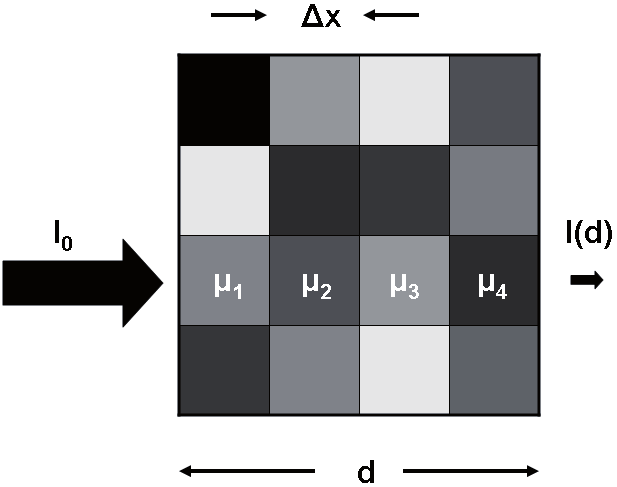
\includegraphics[width=0.5\linewidth]{intro/screenshot001.png}
	\caption{Simplified attenuation matrix (4,4,1); \cite{Maidment2014}}
	\label{fig:voxel_matrix}
\end{figure}

\subsubsection{Hounsfield Units}

In a final CT scan, voxel values are recorded in Hounsfield Units (HU), which relate to the attenuation of water at room temperature:
\begin{align}
HU_{material} = \frac{\mu_{material} - \mu_{water}}{\mu_{water}} \cdot 1000
\end{align}

Table \ref{tab:HU} lists types of human tissue and their values on the HU scale.
Generally, HU values range from -1024 to +3071 (12 bit), but the upper limit can be extended to 15,359 (14 bit) if materials with even higher attenuation need to be visualised (e.g. implants). \\

\begin{table}[]
	\centering
	\caption{Average HU values for various types of human tissue}
	\label{tab:HU}
	\begin{tabular}{@{}ll@{}}
		\toprule
		Substance           & HU                     \\ \midrule
		Air                 & –1000                  \\
		Lung                & –750 (–950 to –600)    \\
		Fat                 & –90 (–100 to –80)      \\
		Water               & 0                      \\
		Muscle              & +25 (+10 to +40)       \\
		Brain, white matter & +25 (+20 to +30)       \\
		Kidneys             & +30 (+20 to +40)       \\
		Brain, grey matter  & +35 (+30 to +40)       \\
		Blood               & +55 (+50 to +60)       \\
		Liver               & +60 (+50 to +70)       \\
		Compact bone        & +1000 (+300 to +2500)  \\ \bottomrule
	\end{tabular}
\end{table}

Typically, CT scans are displayed on Computer monitors, which imposes the need to map the HU values to a 8-bit greyscale (256 steps of luminosity).
Since the number of possible values (dynamic range) on the HU scale is 16 times the shades of grey on a screen (12-8 = 4 bit difference; equivalent to a factor of $2^4$) the screen cannot convey all details at the same time.
A linear mapping would result in 16 neighbouring HU values being compressed to the same brightness on the sreen.
This way, the brightest (bone) and darkest parts (soft tissue) of the image would be clearly distinguishable.
At the same time small differences (<16 HU) would appear to have exactly the same intensity.
However, most of the time, the doctor's focus might lie either on soft tissue or bone material.
Bearing in mind that soft tissue values range only from 10 HU to 70 HU at most (see table \ref{tab:HU}), such a compression would make distinguishing tissues using CT very unreliable.
Instead of showing detail from the lowest to the highest value, a range of values - a so called window - can be chosen.
Let's assume, for example, a range from -100 to 155 HU to be of interest.
This selected range can be mapped directly and uncompressed to a 8-bit greyscale.
Any values above 155 HU will be assigned the brightest value (white = 255), below -100 the darkest (black = 0).
While showing very good soft tissue contrast, all bones would be depicted with exactly the same brightness (255), even though they might have a varying HU values.
For bone structures, a range from 300 to 2500 HU might show sufficient contrast.
Standard computer programs used to display CT images allow the user to change the window interactively to any value range. \cite{Podgorsak, Maidment2014}

\subsubsection{Image acquisition}
The time necessary to collect 1-D attenuation projections from sufficient angles is called 'acquisition time'.
In 2-D X-ray scanning only one picture is taken, while a 3-D CT model is made up of a photo sequence.
If the patient moves during the imaging process, the final model would show motion artefacts which might lead to wrong conclusions.
Consequently, CT scanners are designed to minimise acquisition time while ensuring sufficient image quality.
Very fast CT protocols result in smaller resolution, because less images are taken.
It has to be said, though, that CT acquisition time is usually already significantly shorter than MRI. \cite{Podgorsak, Maidment2014}

\subsubsection{Image quality} %282
Additionally to the relatively short acquisition time, CT scans show little distortion compared MRI (see \ref{sec:MRI}), which is why they are often used as 'gold standards' (reference scans used for MRI distortion assessment).

While bone structures are clearly visible in CT scans, 'soft tissue contrast' is relatively low compared to MRI.
In other words, parts of the body which are considered as 'soft tissue' (intestines, brain, blood vessels, etc.) differ little in brightness and are therefore hard to distinguish.
See \ref{sec:soft} for more information.

Another aspect of image quality is the 'low contrast resolution' of the scan.
It directly relates to how much structures and their surroundings have to differ in signal intensity to be clearly distinguishable by doctors.
The quality of the 'low contrast resolution' is mainly limited by noise.
Noise is a random pattern underlying the actual signal and is always present to some extent.
It's prominence in the final image is described by the Signal to Noise Ratio (SNR).
If the SNR is too low, fine structures blend with the noise and cannot be distinguished. 
Strategies to achieve a high SNR include raising the initial photon flux (intensity) or employing contrast agents.
The intensity is governed by the tube current, which is limited by the heat capacity of the tube and health considerations regarding the patient dose.

Alternatively, the spatial resolution can be decreased, effectively combining neighbouring image slices.
This way the SNR for the combined slices is increased, but fine structures along the z-axis might be lost due to the reduced resolution. \cite{Podgorsak, Maidment2014}

\subsubsection{Health considerations}
CT scans describe the attenuation throughout a patient, which is directly related to how much energy is transferred from photons to matter.
Only because X-rays are absorbed by the human body, this imaging modality gives insight in the density distribution of a body's interior.
However, this transferred energy is capable of causing biological damage. (see \ref{sec:irradiate})

While the radiation dose administered during a single CT scan is relatively small (typically not more than 15 mSv) and almost negligible compared to the dose administered during a potential radiation therapy, patients receiving this dose regularly end up with a potentially harmful accumulated amount of radiation.
Cancer patients, for instance, need to be imaged frequently during treatment planning.
However, patients might die before those consequences come into effect.
Therefore, it's typically children (who received a great number of CTs) to suffer from induced cancer occurring up to 40 years later.
So while the benefit from using CT for diagnostics far outweighs the damage, there have been major efforts to reduce dose while maintaining reasonable image quality.
\cite{Murphy2007, Brenner2001, Sodickson2009, Smith2007, McCollough2009, Goldman2013}


\subsection{Magnetic Resonance Imaging - MRI}
\label{sec:MRI}
Magnetic Resonance Imaging (MRI) is a 3-D imaging modality based on Nuclear Magnetic Resonance (NMR), a phenomenon discovered by physicist Isidor I. Rabi in 1938.
Atomic particles such as protons have an inherent quantum mechanic feature called 'spin', which is associated with a magnetic moment $\mu$.
Without an external field, a proton's spin is oriented in a random direction in space and so is its magnetic moment.
The sum of magnetic moments belonging to a number of protons results in a net magnetisation.
Due to their random orientation, the net magnetisation will be zero for a sufficiently high number of particles.
This is because, on average, for every proton's spin there is always another particle's spin oriented exactly the opposite way cancelling its magnetic moment.

In the case of an applied external magnetic field (this static field is often called B0), the spins will either align parallel (pointing in the same direction) or anti-parallel (opposite direction) to this field, where their energy reaches a local minimum.
Parallel protons have an even lower energy than those pointing the other way.
In a collection of many spins, the number of parallel spins will therefore slightly dominate, resulting in a net magnetisation greater than zero (see figure \ref{fig:spin_align}).
In other words, only the amount of protons that is not compensated by those looking in the opposite direction contributes to a detectable magnetic field.

\begin{figure}[h!]
\centering
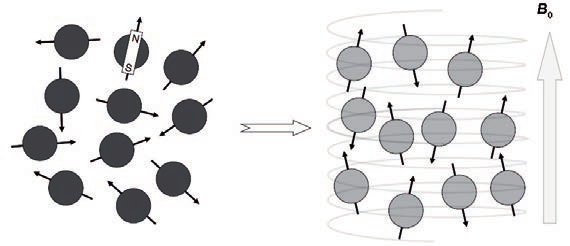
\includegraphics[width=0.8\linewidth]{../fig/intro/spin_align}
\caption{The spins, initially oriented randomly in space, become aligned either parallel or antiparallel to an externally applied magnetic field $B_0$. \cite{Maidment2014}}
\label{fig:spin_align}
\end{figure}

By applying a short radio frequency pulse (often referred to as B1), the total external magnetic field changes and the magnetic moments start precessing around that new external field.
The pulse duration is usually chosen as to flip the spins by a $90^o$ angle.
They are now oriented in the transverse plane to the original external field, and so is the resulting net magnetisation.
Similar to how a spinning top rotating at an angle to the direction of gravity precesses, the magnetic moments will now precess about the direction of the external field with a frequency linearly proportional to the external field strength.
This precession movement can be detected as induced current in a receiver coil, because the net magnetisation still follows the spins' orientation. 
Again, the particles would like to minimise their energy by aligning their spins to the external field, but in order to do so they need to give away the surplus energy, transferring it to the surrounding lattice.
Those spin-lattice interactions happen with different efficiency depending on the tissue.
The time it takes the spins to align is expressed in a material specific time constant $T_1$.
Shortly after applying the radio frequency pulse, regions of the body where magnetic moments align quickly (short $T_1$) have a stronger net magnetisation (in the direction of the external field) than those where energy is being transferred slowly (long $T_1$).

At the same time, the spins interact with each other, affecting the local magnetic field and spins in their vicinity.
The magnetic moments, which started out precessing in phase directly after the radio frequency pulse flipped them, will precess at slightly different frequencies, due to the small fluctuations of the local magnetic field.
The differences cause the collection of magnetic moments to 'de-phase' and the net magnetisation in the transverse plane to vanish.
This process caused by spin-spin interactions is described by the material specific time constant $T_2$.
Eventually, all spins will be again aligned either parallel or anti-parallel to the external field, just as they were before the RF-pulse.

Applying the RF pulse with a homogeneous field strength along the whole body would excite all spins simultaneously.
In order to localise differences in tissue magnetisation, the RF pulse is instead combined with a linear magnetic gradient field 'selecting' a slice to be imaged at a time.
The rest of the body is unaffected, the signal measured directly after such a pulse was applied originates only from the chosen slice.
Eventually, by collecting data on the net magnetisation throughout the body in different locations ('scanning' the patient slice by slice), a 3-D image can be computed.

Depending on the information required from the examination, Doctors can choose to create images that reflect spin-lattice interactions ($T_1$ weighted) or spin-spin interactions ($T_2$ weighted).

Governed by the chosen settings, particular tissues will displayed varying contrasts.
For example, areas with increased water level will be dark on T1 weighted ($T_1w$) MRI whereas the same areas will be bright on $T_2w$ MRI.
Additionally, certain types of materials (tissues) can be intentionally not imaged (suppressed) to reveal others that are in their close proximity.
This is often done with fatty tissue that can cover relevant parts of the field of view.
There are various methods how this can be achieved.
MR imaging gives practically endless possibilities in terms of selective imaging and is mostly limited to imaging time and technical characteristics of the scanner.
Medical physicists and scanner vendors are incessantly working on new MR imaging methods and applications. 

The set of parameters governing how the tissue is excited and data acquired is called 'image sequence'.
Delineating tumours or lesions is often accomplished by looking at both $T_1w$ and $T_2w$ weighted images and drawing the right conclusions.

Soft tissue contains a lot of water, which is made up by oxygen and hydrogen.
Hydrogen nuclei are single protons and their nuclear magnetic resonance is what MRI is tuned to visualise.
This is why soft tissue appears as bright areas in MRI, whereas bone material has only little contrast. \cite{Currie2013}


Most the scanners are build to house a receiver coil in the gantry and they are able to measure the signal using only this one coil.
However, a stronger signal could be obtained by placing the coil closer to its source, the patient.
As the region of interest (ROI) is usually limited to a specific organ, receiver coils are available in different sizes and shapes, often designed to fit the patient with a comfortable but narrow space in between.
To get even closer, so called 'surface coils' can be placed on the patient.
'Spine coils' are sometimes hidden in the table on which the patient lies during the examination.
Typically, for creating images of a patient's head, coils with a fixed arc-like geometry are used.
This type of coil was also used for the data acquisition of this thesis.

Studies have shown that delineating certain types of tumours, for example prostate cancer, is more accurate using MR images than using CT. \cite{Rasch1999, Debois1999a, Roach1996}

In diagnostics, MR images prove to be very useful.
Also for radiation therapy treatment planning, the superior soft tissue contrast is exploited during the definition of organs at risk and targets.
Unfortunately, due to the physical principles of MRI, it indirectly provides the information about the proton density, whereas CT can provide information about electron density.
It is knowledge of the electron density which is necessary in the treatment planning process.
During this, the dose distributions are calculated based on the applied beam geometry and the distribution of matter on its way.


\subsubsection{Image Quality}
Contrary to CT, MRI is prone to distortion due to field inhomogeneities.
Organs might appear shifted, elongated or shrunk.
The effect is most prominent along the outer edges of the scanner's field-of-view (FOV).
In the isocentre (middle) of the scanner, the distortion is smaller, because here the field is least aberrant.
For most applications, small position shifts and deformations are of minor importance.
MRI scanners usually come equipped with an internal distortion correction algorithm.
Figure \ref{fig:dist_compare} shows the unmodified and the corrected version of an image coming from such a scanner.
Those methods are developed by the company designing the scanners.
Knowing the technical details enables them to write tailor-fit scripts which drastically reduce the distortion.

However, for Radiotherapy treatment planning this might not be enough and it is necessary to additionally monitor the distortion and, if necessary, take additional corrective measures. 

While its soft tissue contrast is superior to CT, a relatively long acquisition time is necessary to achieve a sufficient high SNR.
This leads to the risk of motion artefacts (patients moving during the scanning procedure).
To tackle this issue, resolution can be reduced, effectively combining signal from several voxels to create a single voxel, reducing the overall noise.
The trade-off is that fine structures might get lost.

\begin{figure}[h!]
\centering
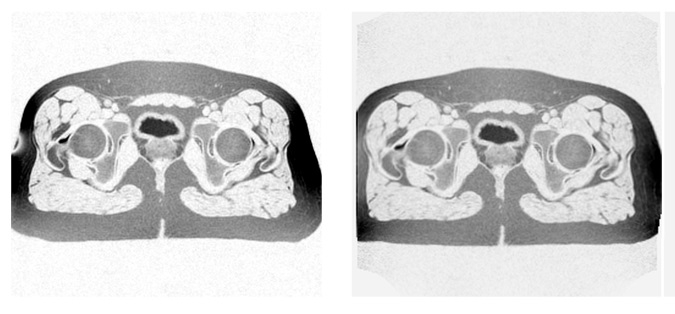
\includegraphics[width=\linewidth]{../fig/vgl-corr_inverse.jpg}
\caption{On the left is the original image, on the right the automatically corrected version of the same MR image (inverted colours)}
\label{fig:dist_compare}
\end{figure}

%Field of view (FOV) of the MRI scanner is smaller than the CT scanner's.


\subsubsection{Health considerations}

Strong, static magnetic fields (typically up to $3T$) are present around MRI scanners at all times, and precautions have to be taken to ensure safety for patients and medical personnel.
Ferromagnetic materials (such as steel and iron) can become dangerous projectiles in vicinity of the MRI scanner.
They must be excluded from the room housing the magnet without exception.\\

%It is also important to remember that medical implants, including but not restricted to cardiac pacemakers and hearing-aids, might malfunction or become damaged in strong fields regardless whether they contain ferromagnetic materials.
%Patients with such implants might still be imaged with scanners utilising weak fields up to $0.5T$.

The RF pulses repeatedly put spins in excited states, transferring energy to the human body.
MRI scanners are designed to limit the rise of a patient's body temperature to $0.5^oC$ during standard imaging.
Only combined with either medical or appropriate psychological monitoring the limit can be raised to $1^oC$.
An ethics committee approval is necessary for even higher values.
In general, patients should be exposed to RF fields only as strong as their thermoregulatory system is capable to cope with.\\

Finally, magnetic field gradients are applied together with the RF pulse.
They are switched at high frequencies leading to induced currents in conducting body tissue.
In principle, those currents stimulate nerves which might result in muscle twitching or pain.
However, gradient levels are set to avoid stimulation.
During have reported some subtle biological effects, but there was no evidence pointing towards harm caused by short term exposures.
At the same time, patients suffering from epilepsy might show increased sensibility to induced electric fields in the cortex and should be imaged with caution. \cite{Maidment2014}
Some patients might be allergic to contrast agents used for specific MRI examinations.
Here, safety procedures are similar to those performed during administration of regular drugs. 

\subsubsection{Open bore MRI scanners}

The radiation oncology department of the Vienna General Hospital (AKH) is equipped with an $0.35  T$ open-bore, c-arm MRI scanner (see Section \ref{sec:magnetom} for more details).
This open design has proven to drastically improve the well-being of patients experiencing anxiety in closed-bore scanners.
For this reason, the number of incomplete MR examinations due to a claustrophobic events is relatively low. \cite{Enders2011a, Bangard2007}
Besides, patients who would not fit in closed designed scanners can be imaged.
Furthermore, brachytherapy patients can be placed in the scanner with applicators attached (see chapter \ref{sec:brachy} for more details).

This scanner's magnetic field is weaker than the fields of closed-bore scanners that are widely used (typically 1-3 Tesla).
High field strengths result in greater resolution, better Signal to Noise (SNR) ratio and faster imaging time.
Generally, diagnostics benefit from greater image quality.
However, at some point, diagnostic accuracy stops increasing with field strength.
At the same time significant improvements can be achieved at low fields.
A ``combination of field independent polarisation [...] with frequency optimized MRI detection coils [...] results in low-field MRI sensitivity approaching and even rivalling that of high-field MRI.'' \cite{Coffey2013}

Low field MRI scanners are also typically characterised by less distorted images. \cite{https://link.springer.com/article/10.1007/PL00002385}

Apart from the often satisfactory image quality, there are considerable cost advantages to the use of lower field MRI.
The initial purchase price and the ongoing maintenance expenses are considerably lower than those of high field scanners, which often use superconducting magnets cooled with liquid helium. \cite{Rutt1996}
Permanent magnets might be weaker, but do not require constant cooling.
Also, low fields allow facilities to build smaller rooms and magnetic objects are less dangerous.


\subsubsection{Diffusion Weighed Imaging - an example for non morphologic Imaging}

Despite the fact that this type of MR imaging was not used for this thesis, it will be mentioned here as an example of the vast range of measurements possible with MRI techniques.\\

% https://www.youtube.com/watch?v=J_aamnpRJE8
% mri - from picture to proton S. 331 (im pdf auf 344)
Diffusion weighted (DW) imaging quantifies molecular diffusion in the body.
This imaging technique uses MRI technology differently:
Additionally to the gradients needed to select a slice (strength $~3-5\, mT/m$, duration $2-4\, ms$), the sequence for DW imaging applies two long, strong, consecutive and opposite gradients (strength $~30-50\, mT/m$, duration $20\, ms$) during which molecules may move due to diffusion.
After those two gradients (which, usually, will be applied in all three Cartesian directions), the remaining signal (net magnetisation) is measured by the receiver coil.

Molecules which are restricted in their movement will experience two equally strong but opposite magnetic fields.
The first will cause them to precess with a certain speed (linear with field strength), effectively changing their phase.
The second will cause them to precess exactly the other way around (same strength, but other direction), returning them to their initial state.
Now they will again be in phase and result in a net magnetisation which is not zero, but visible as bright areas on the scan.

Those molecules which are free to move, however, will not experience a constant field strength, because the field has a gradient.
As they move through the body they will precess at varying speeds during the first and then at different speeds during the second gradient.
As a result, they will be out of phase when the net magnetisation is measured by the receiver coil, and will not cause bright areas in the scan.

DW imaging can be used to diagnose acute strokes (brain infarct), because areas with restricted diffusion (blocked blood flow) show a strong signal compared to healthy tissue with normal diffusion.
Another interpretation of low diffusion (high measured signal) can be the increased cellular density (so dense that free diffusion of water molecules is suppressed) which is characteristic for cancerous tissue.\\

Since the time necessary to allow the molecules to move during the two gradients is relatively long, the image will naturally be $T_2$ weighted.
This is taken into account by creating a second image which is also $T_2$ weighted, but does not apply two consecutive opposite gradients.
The difference between the DW and the not DW weighted sequences reflects the actual contribution of diffusion (apparent diffusion coefficient - ADC).


\section{Radiation therapy}
\label{sec:planning}
Radiation therapy utilizes ionizing radiation to damage and kill cancer cells in order to stop them from multiplying.
This prevents the growth of tumours, makes them shrink in size and hopefully cures the patient. 

During radiotherapy treatment planning (RTP), 3-D models of the patient are used to define targets (regions where the dose should go) and organs at risk (where the dose should not go).
This ensures that vulnerable organs are spared from radiation while making sure the tumours receive sufficient dose.
Moreover, methods to quantify the amount of radiation that different body parts absorbed are needed, because the actual treatment might differ from the plan.\\

While travelling through matter most types of radiation release energy mainly due to coulomb interactions with the outer shell electrons of atoms.
Knowing the electron density of the targeted tissue area is therefore essential.
In order to reach a specific penetration depth, the particles' initial energy has to be chosen accordingly.
The necessity to treat the tumour with a required amount of radiation leads to a radiation therapy treatment plan.

There are two well established methods for applying the radiation.
External beam radiotherapy (EBRT) is performed from afar:
Gantries are able to position the radiation source around the patient in a way covering virtually any possible angle.
During a treatment session, fractions of the total dose are administered from many different locations.
The sum of those individual treatments results in the required dose distribution.
Figure \ref{fig:plan} shows an example of two differently calculated treatment plans.

In conventional EBRT, photons (X-rays) in the range of 4MeV to 20MeV are used to deposit the necessary dose at the location of the tumour.
Unfortunately, radiation interacts with all cells it passes until it is fully absorbed.
It releases its energy along its entire path while travelling through the patient.
This behaviour may result in energy being transferred to cells all the way from the point of entry to the point where the (weakened) ray leaves the patient.
Other types of ionising radiation are also used, but less common.
Electrons and low energy X-rays are favoured for some superficial tumour; rare methods using neutrons and even muons also exist.
Charged particle therapy (using e.g. protons or carbon ions) is on the rise, but far from reaching the popularity of X-rays.
This type of radiation minimises the damage done to healthy tissue due to its distinctive behaviour in energy loss called ``Bragg Peak''.
They release most of their energy only shortly before being stopped completely.
\cite{Nakamura2010} This effect can be used to spare tissue lying behind the tumour from radiation entirely and also reduce the amount of energy transferred to organs located before. \cite{Paganetti2005}
A comparison between the behaviour of X-rays and protons is shown in figure \ref{fig:bragg}.\\

Brachytherapy, on the other hand, is when the radiation source is placed close to or inside of the patient.
The source is either moved close to the target area using applicators (temporary treatment) or implanted permanently.
The latter method is done by inserting so called "seeds" (sealed metal containers with radioactive material) directly into the target area where they release high amounts of radiation.
Over time they become less active and eventually the treatment stops automatically.
These rice grain sized implants can remain in the body without causing any harm.
Treatment of prostate and cervix cancer is often done with this technique.
In comparison to EBRT, Brachytherapy allows higher doses while at the same time minimising the radiation reaching organs at risk; precise dose distributions can be achieved.
At the same time, not all cancer types can be treated this way.
For some, a non-invasive method (e.g. EBRT) is a better alternative.\\


\begin{figure}[!h]
	\centering
	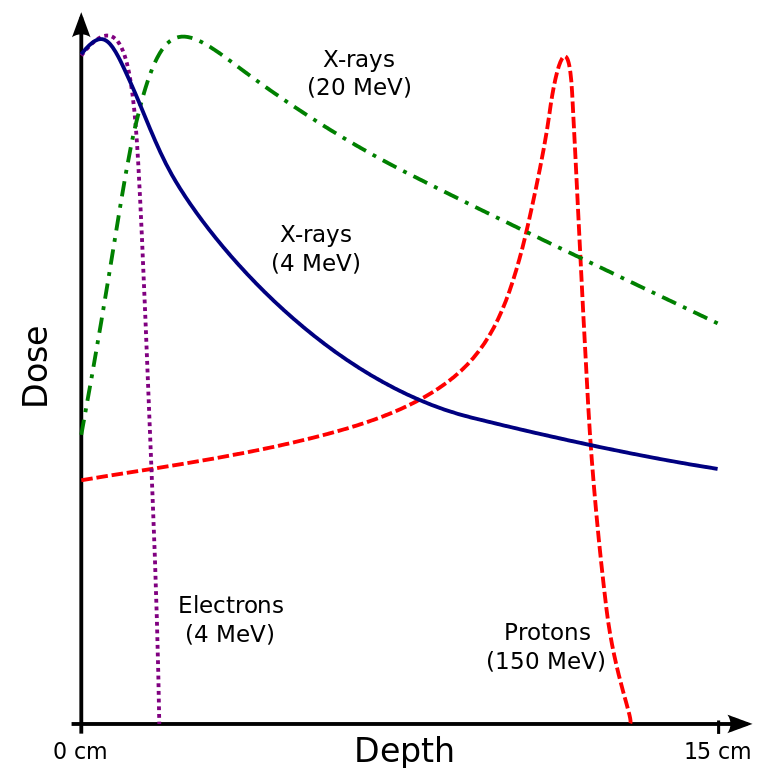
\includegraphics[width=0.6\textwidth]{Dose_Depth_Curves.png}
	\caption{energy release of ionising radiation; \cite{Cepheiden}}
% (By Cepheiden, via Wikimedia Common;\\ GFDL \url{http://www.gnu.org/copyleft/fdl.html})
	\label{fig:bragg}
\end{figure}

\begin{figure}[!tbh]
	\centering
	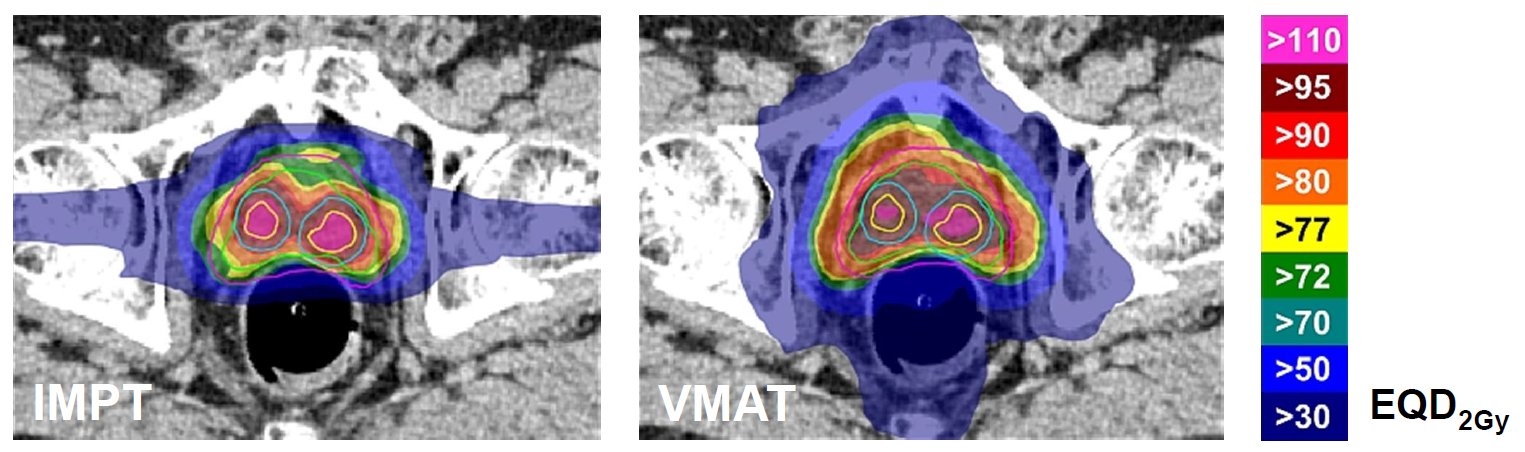
\includegraphics[width=\textwidth]{Plans.png}
	\caption{Example of Radiotherapy treatment plan: coloured areas represent dose values deposited during treatment. The plans were calculated using different planning techniques (IMPT and VMAT). (image source: \cite{piotr})}
	\label{fig:plan}
\end{figure}

\clearpage

%\subsection{Types of radiation therapy}
%\todo{(Based on the IAEA Handbook Radiation Oncology Physics) Tele – is typically delivered in the range of few to some 20MV with linear accelerators (describe briefly the dose depth curve and that to be able to accumulate dose in the target and spare the OAR normally multiple number of beams is combined), typically photons are used but also electrons can be produced to treat superficial targets. For the latter also a low energy X-rays can be utilized – orthovoltage units. Then there are also havier particles to utilize like protons, neutrons or light ions – here few words about the Bragg peak. }


\subsection{Role of CT}

Until recently, radiotherapy treatment planning (RTP) relied almost entirely on CT.
There are two main reasons for this:

Firstly, calculating the electron density using data obtained with CT is an straightforward task.
Secondly, CT images generate 3D images with little distortion. Exact geometries are needed for correct RTP.
It is the most reliable approach to create precise radiotherapy treatment plans. \cite{Constantinou2012, Schneider1996}

\subsection{Role of MRI}
MR images also record luminosity values, but they do not correspond to radiodensity.
Due to the better visibility of tumours on MR images, RTP often uses combined data from both imaging modalities.
Additional information derived from DW MRI can also support response prediction and assessment.
However, there are some difficulties arising from combining CT and MRI for EBRT:
In order to profit from separately acquired data, the resulting images must be aligned (registered) either manually or automatically.
This is a hard task since non-rigid objects (organs) change their shape and location between measurements which may lead to inaccuracies.
Algorithms supporting non-rigid registrations are already under development, but there is still room for improvement.
For now, only local rigid registration is capable of reliable target and organ at risk definition.

Alternatively, MRI-only radiation therapy protocols are being developed:
One way of doing this is to use MRI data to create a Pseudo-CT, which contains information about electron density.
Comparisons to using CTs and MRI-based pseudo CTs have shown acceptable deviations for X-ray therapy.
In charged particle therapy the resulting dose gain in healthy tissue and dose loss in cancer regions owed to inaccurately assigned electron density values is bigger.
However, further improvement of accuracy promises to reduce time and money needed for RTP when CT is no longer needed.
Furthermore, patients would be spared the additional dose of CT examinations.  \cite{Rank2013, Stanescu2006, Nyholm2015, Greer2015, Chen2004}


\section{Aim of this work}
The idea of only using MRI for treatment planning is approaching the clinics, but there are still some issues that need to be addressed.

Due to the possible image distortion, great care needs to be taken and the MR images must be verified before they are used for RT target definition and dose calculation.
The available MRI scanner at the AKH is equipped with an on board correction algorithm which is supposed to reduce distortion.
See figure \ref{fig:rendered_dist} for an example of how this correction affects an image.
Distorted images might lead to wrong calculations of how much energy is needed for the radiation to accumulate exactly at the target region.
If, for example, bone structure is depicted as thicker than it really is, RTP would suggest a treatment which would deposit more energy behind the tumour than intended.
The opposite holds for cases where tissue appears to be thinner, which would result in areas lying before the tumour being irradiated.

The goal of this work is to:
find an optimal (providing satisfactory image quality and convenience of use) liquid filling for the rod cavities in an already existing custom designed distortion phantom provided by the AKH Vienna to be able to acquire the reference CT image and test MR acquisitions.

develop and implement a method to assess and illustrate the distortion of the MR image based on tracking of the distortion of one of the phantom rods, with an option to further extend the tool for mutli-rod tracking.
% develop and implement in silico a method to assess and illustrate the distortion of the MR image based on tracking of the distortion of one of the phantom rods, with an option to further extend the tool for mutli-rod tracking.

Therefore, this work focuses mainly on the assessment of the acquired imaging data (using the implemented software tools), choosing which liquids to fill the phantom with, but not its entire design.
However, possible fillings have to be produced and tested.
Similar approaches are being used for distortion correction by other facilities. \cite{Price2015, Petersch2004, Torfeh2015, Wang2004, Wang2004b, Mizowaki2000}


\begin{figure}[!thb]
\centering
  \begin{subfigure}[b]{0.49\textwidth}
  \centering
    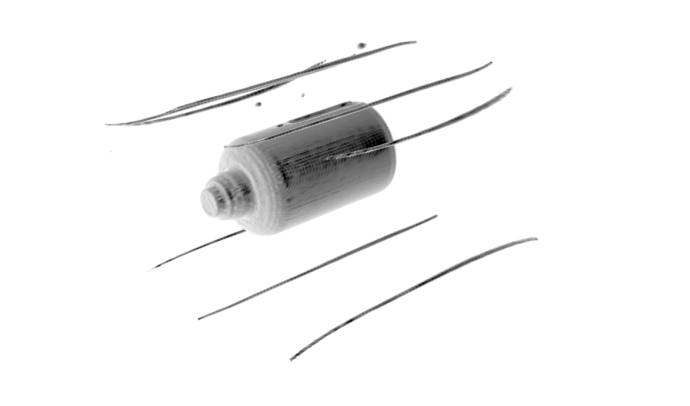
\includegraphics[scale=1.2]{rendered/rendered_MR.png}
    \caption{MR scan with no distortion correction}
    \label{fig:rendered_MR}
  \end{subfigure}
  \begin{subfigure}[b]{0.49\textwidth}
  \centering
      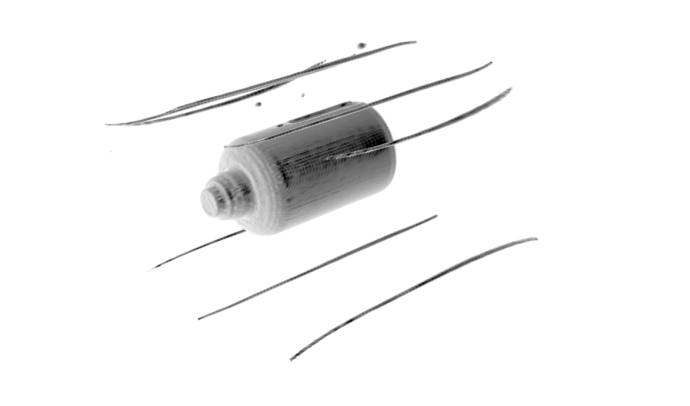
\includegraphics[scale=1.2]{rendered/rendered_MR_corr.png}
    \caption{MR scan after internal distortion correction}
    \label{fig:rendered_MR_corr}
  \end{subfigure}
  \caption{Rendered MR scan showing the difference before (a) and after (b) applying the build-in distortion correction.}
  \label{fig:rendered_dist}
\end{figure}


%to me \footnote{Auszug aus \citetitle{BohemRhap}~\cite{BohemRhap} von \citeauthor{Queen}~\cite{Queen} }\\
%\section{Farrokh Bulsara aka. Freddie Mercury}
%Weitere Zitate sind in Anhang \ref{appendix:zitate} zu finden.